\chapter{Analysis}

\section{Introduction}

\subsection{Client Identification}

My client is Josh Campbell, he is 24 years old. He uses computers regularly for deisgn work, so has experience of computer systems. He uses his computer to design flyers, handouts, banners and visual graphics for projection, as well as surfing the web, email and various social media networks.He rarely uses hard copies other than to preview hes work before sending it off to print. Josh uses a 2012 Mac Pro with the latest version of Apple's operating system, OS X (10.9).\\

\noindent Josh is the head of the media department for Cambridge Community Church. This involves being responcible for the large amount of Audio and Visual equipment used on the churches Sunday services. This currently invloves spreadsheet with limited info on each item. \\

\noindent Josh would like to have a database management system to be able to hold information about each item and their various attributes. He would likke this database to be lovated on the churches central server so that it can be accessed by all staff if it it deemed necessary. He would use this database to store location, value and insurance details incase of damage or theft.he would like all of the information kept as a virtual copy as well as a hard copy to kept as a visual backup in case of harddrive failure or corruption. He would also like to keep the location of each item as up to date as possible and if the location changes, he would like to be notified by email when it is entered/updated in the system.

\subsection{Define the current system}

The current system consists of multiple excel spreed sheets. There is one spread sheet for each of three locations; main office, main church building, and storage. Each spreedsheet consists of items located there as well as information on the value of each item, the quantity and the total value for the items with multiple entries. Each spreedsheet is divided up into equipment type (i.e Cableing, lighting, audio, visual/camera's) 

\subsection{Describe the problems}

There are a number of problems with the current system. One of the problems is that there is no notification system to tell you when information is getting outdated or something is changed. For example, if an item is bought or sold, the total costings for that item will be updated and no-one will be notified. Another problem is that the current system doesn't show the PAT testings for all the items, these tests go out of date every 6 months and there is no way of being notified when a new PAT test is needed on an item.

\subsection{Section appendix}

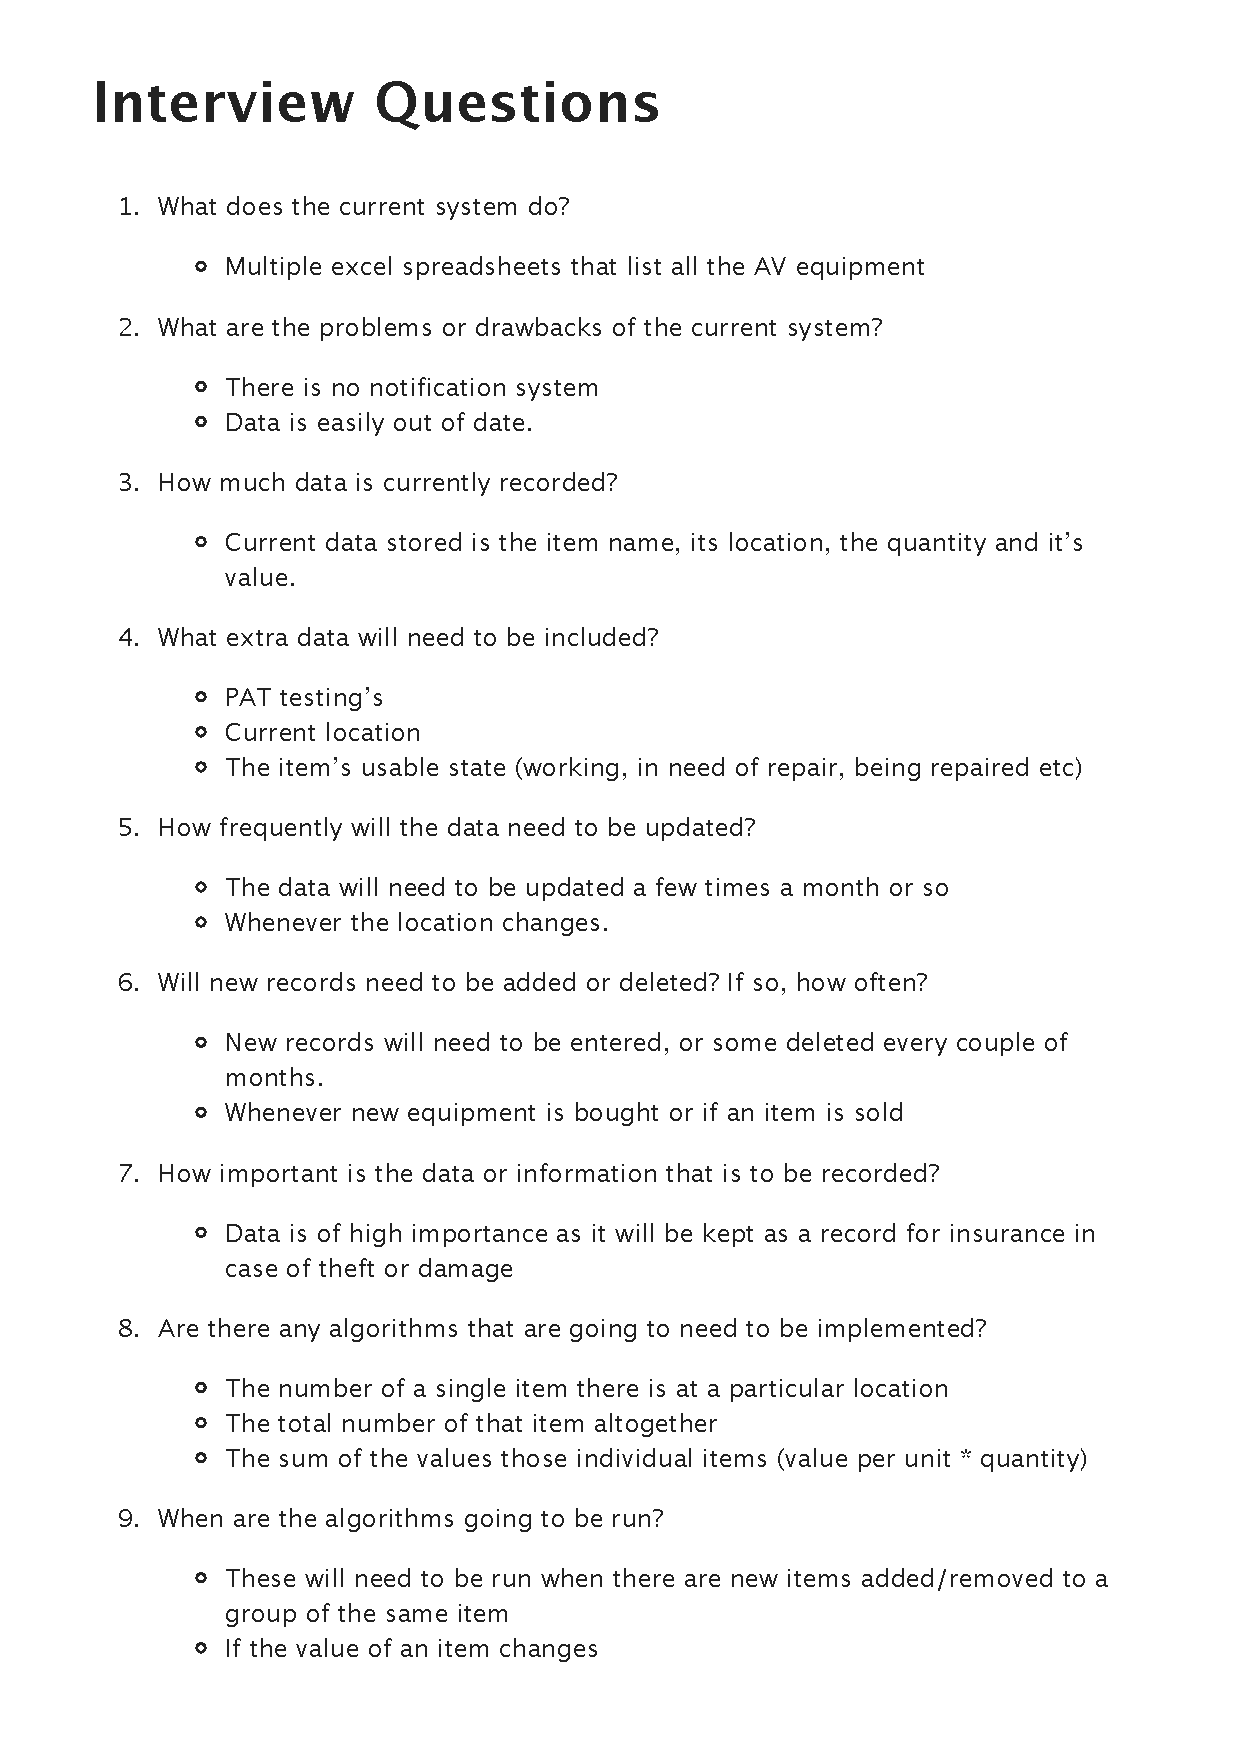
\includepdf[pages=-]{./Analysis/Interview/interview_questions.pdf}
\section{Investigation}

\subsection{The current system}

\subsubsection{Data sources and destinations}

In the current system, there are multiple data sources. The client and his colleagues as well as members of the AV crew for the church can enter data into the spreadsheet by using a computer in the office and accessing the on the server.

\subsubsection{Algorithms}

In the current system, there are only a few algorithms in place.
\bigskip

\begin{algorithm}[H]
    \caption{Algorithm 1, When new item is bought:}
\begin{algorithmic}[1]
\If{$Item = NewItem$}
    \SET{$Action$}{$Enter New Item$}
\ElsIf{$Item = ItemMatch$}
    \SET{$Action$}{$Update Item$}
\EndIf
\end{algorithmic}
\end{algorithm}

\begin{algorithm}[H]
    \caption{Algorithm 2, When an item is sold or replaced:}
\begin{algorithmic}[1]
\If{$Item = Sold$}
    \SET{$Action$}{$Update Quantity$}
\ElsIf{$Item = Damaged$}
    \SET{$Action$}{$Update Quantity$}
    \SET{$Action$}{$File Insurance Claim$}
\ElsIf{$Item = Stolen$}
    \SET{$Action$}{$File Insurance Claim$}
\EndIf
\end{algorithmic}
\end{algorithm}

\subsubsection{Data flow diagrams}

\begin{figure}[H]
    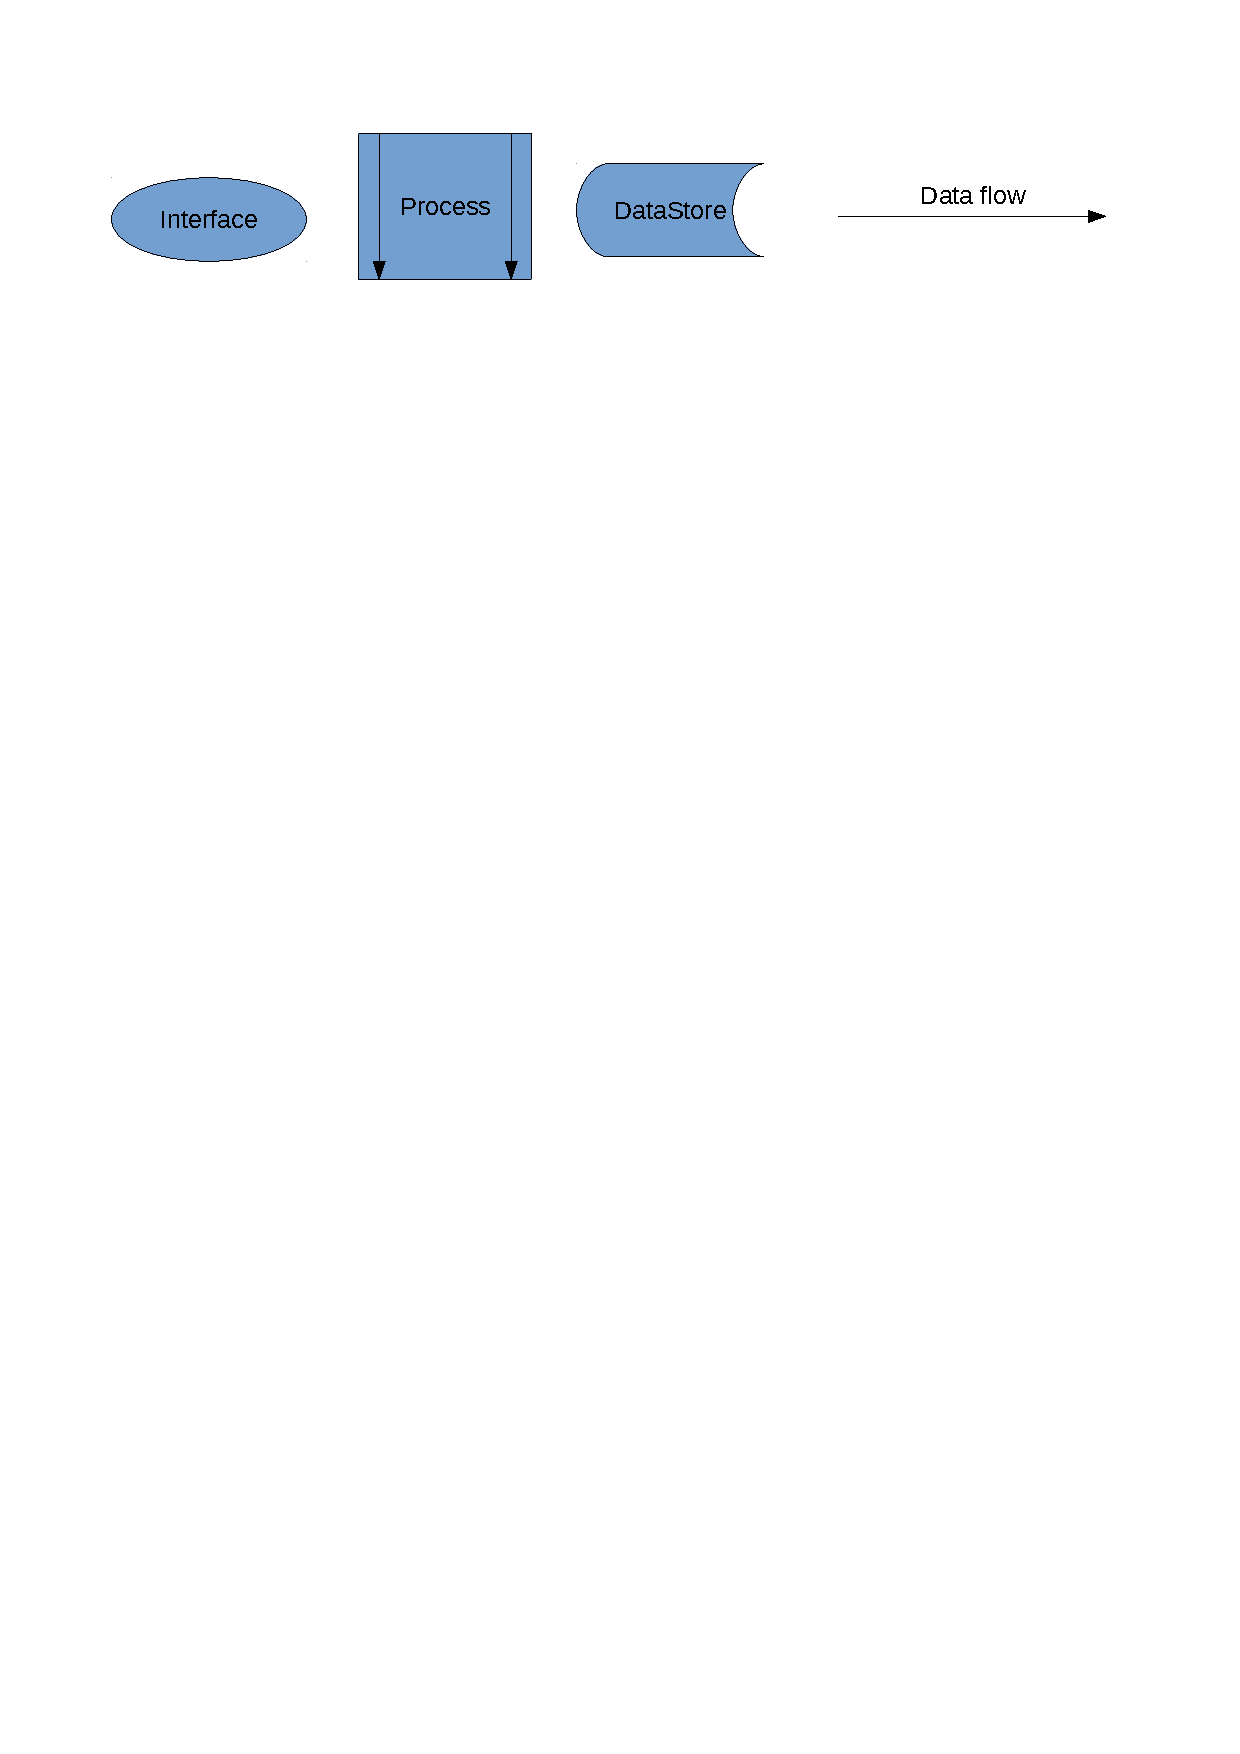
\includegraphics[width=\textwidth]{./Analysis/Dataflow/DFD_analysis_key.pdf}
    \caption{Flow Diagram Key.} \label{fig:print_function_result}
\end{figure}

\begin{figure}[H]
    \centerline{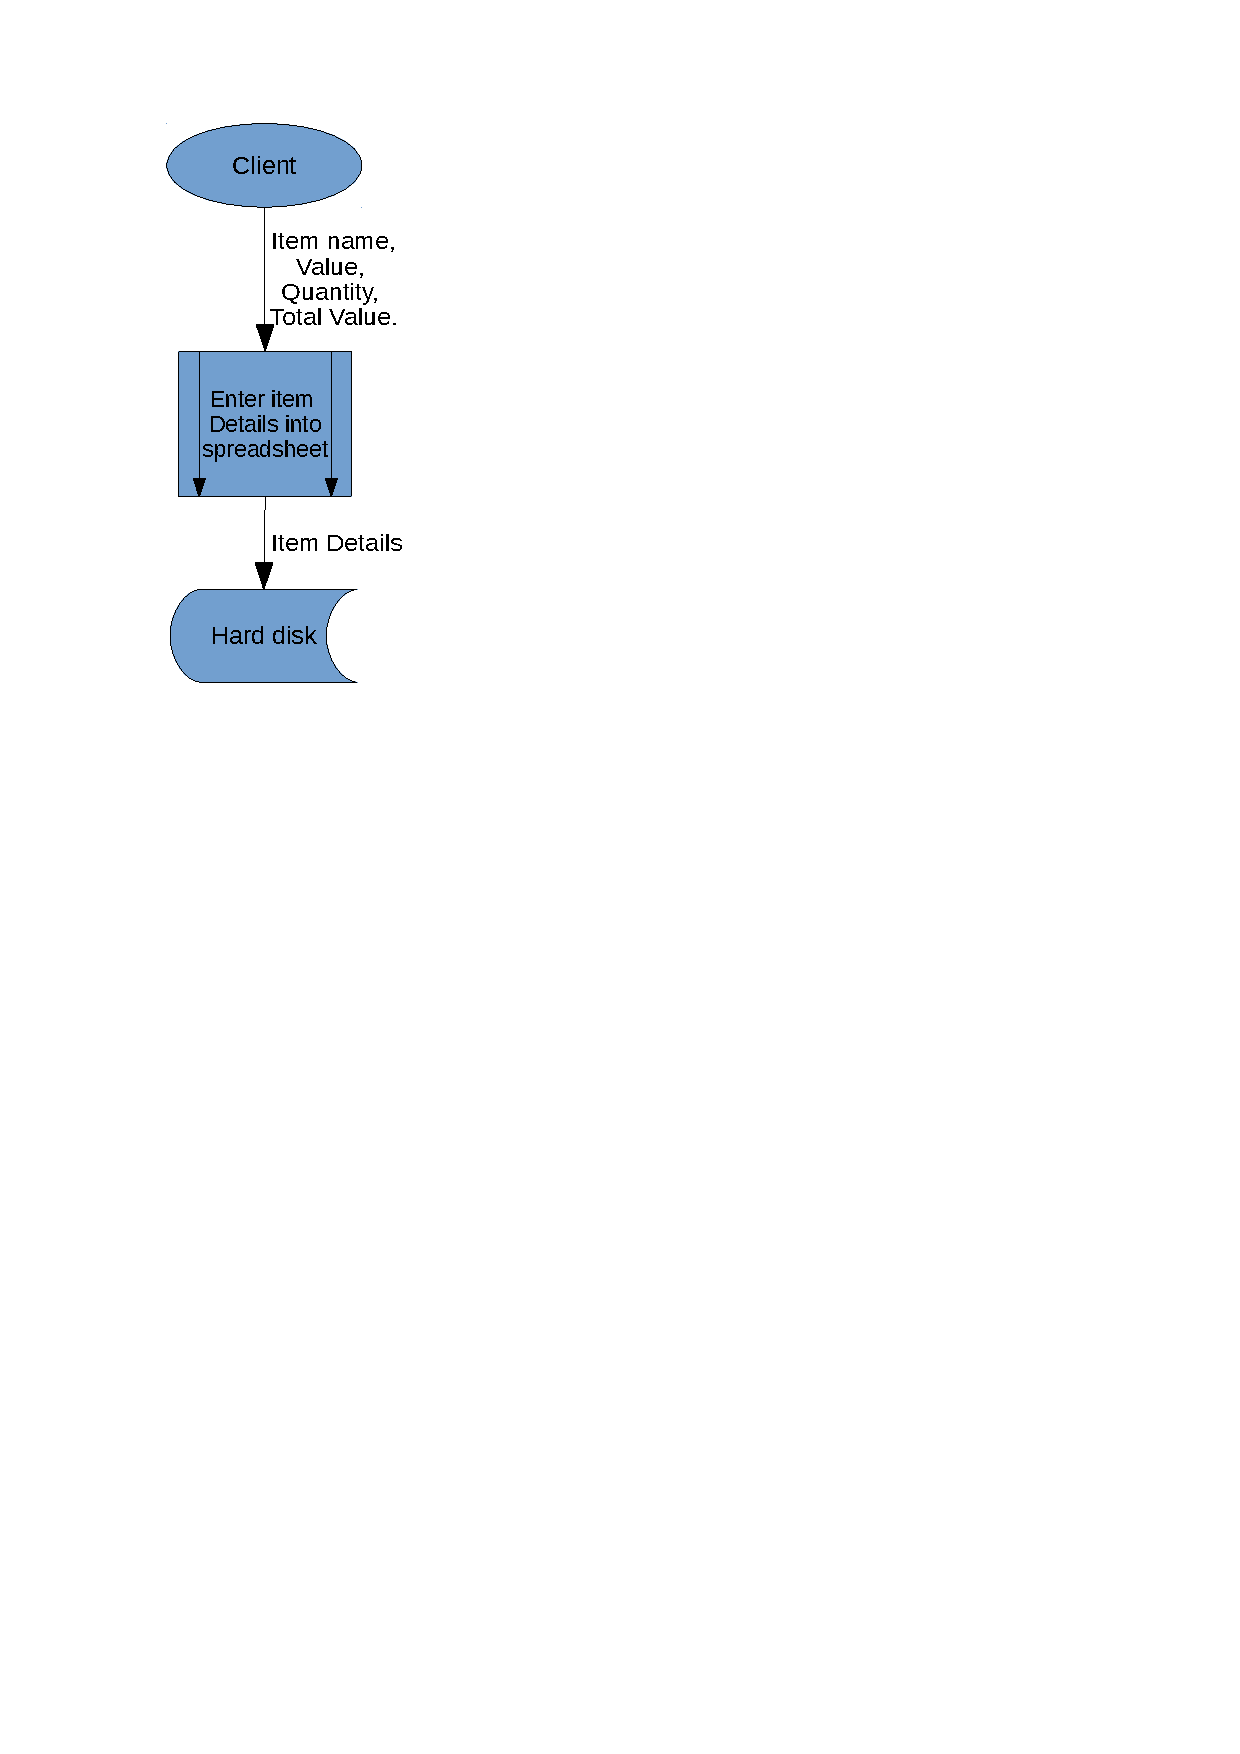
\includegraphics[width=130px]{./Analysis/Dataflow/DFD_analysis_new_item.pdf}}
    \caption{Entering a new item.} \label{fig:print_function_result}
\end{figure}

\begin{figure}[H]
    \centerline{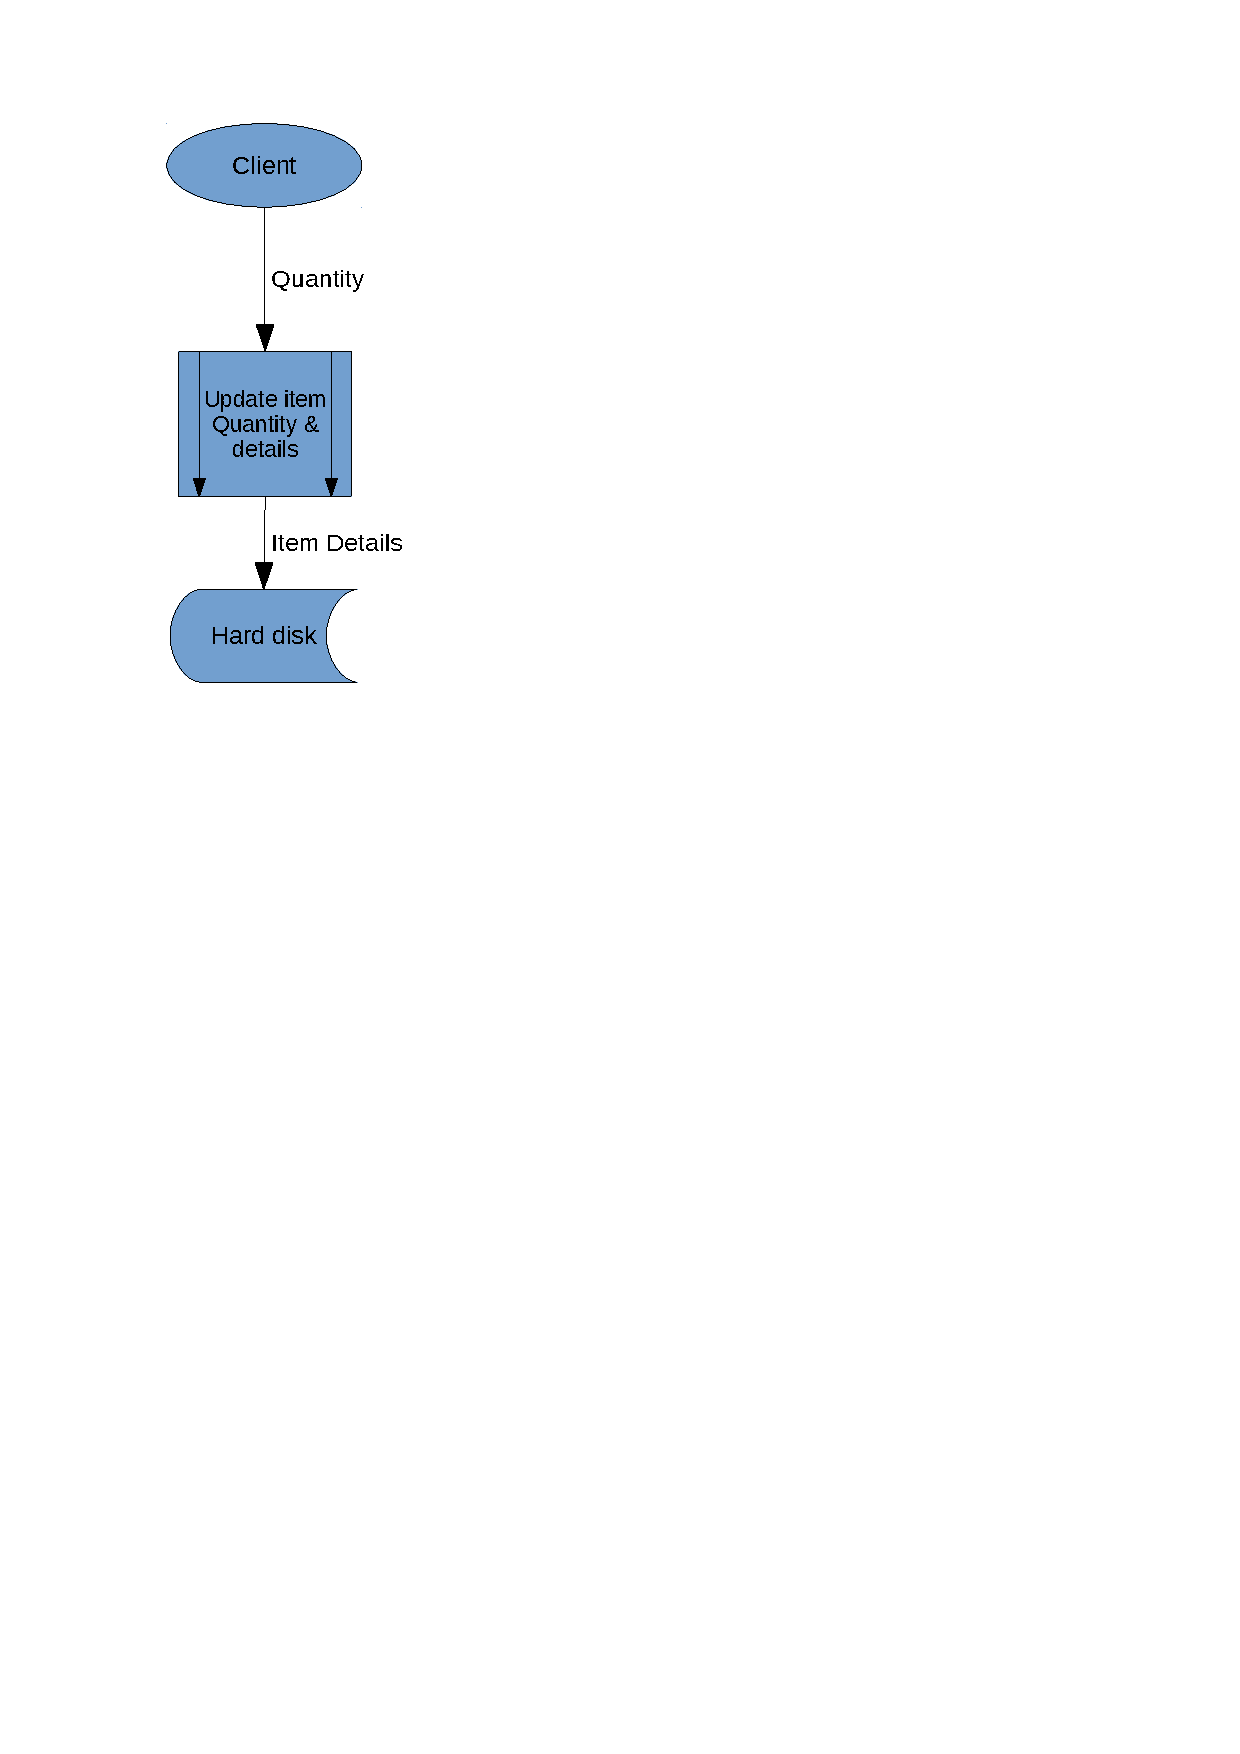
\includegraphics[width=125px]{./Analysis/Dataflow/DFD_analysis_update_item.pdf}}
    \caption{Flow Diagram Key.} \label{fig:print_function_result}
\end{figure}

\newpage

\subsubsection{Input Forms, Output Forms, Report Formats}

Josh has provided me with a screenshot of him entering some data into his current system. I have boxed out confidential information such as item values and their respective sub-total values:\\

\begin{figure}[H]
    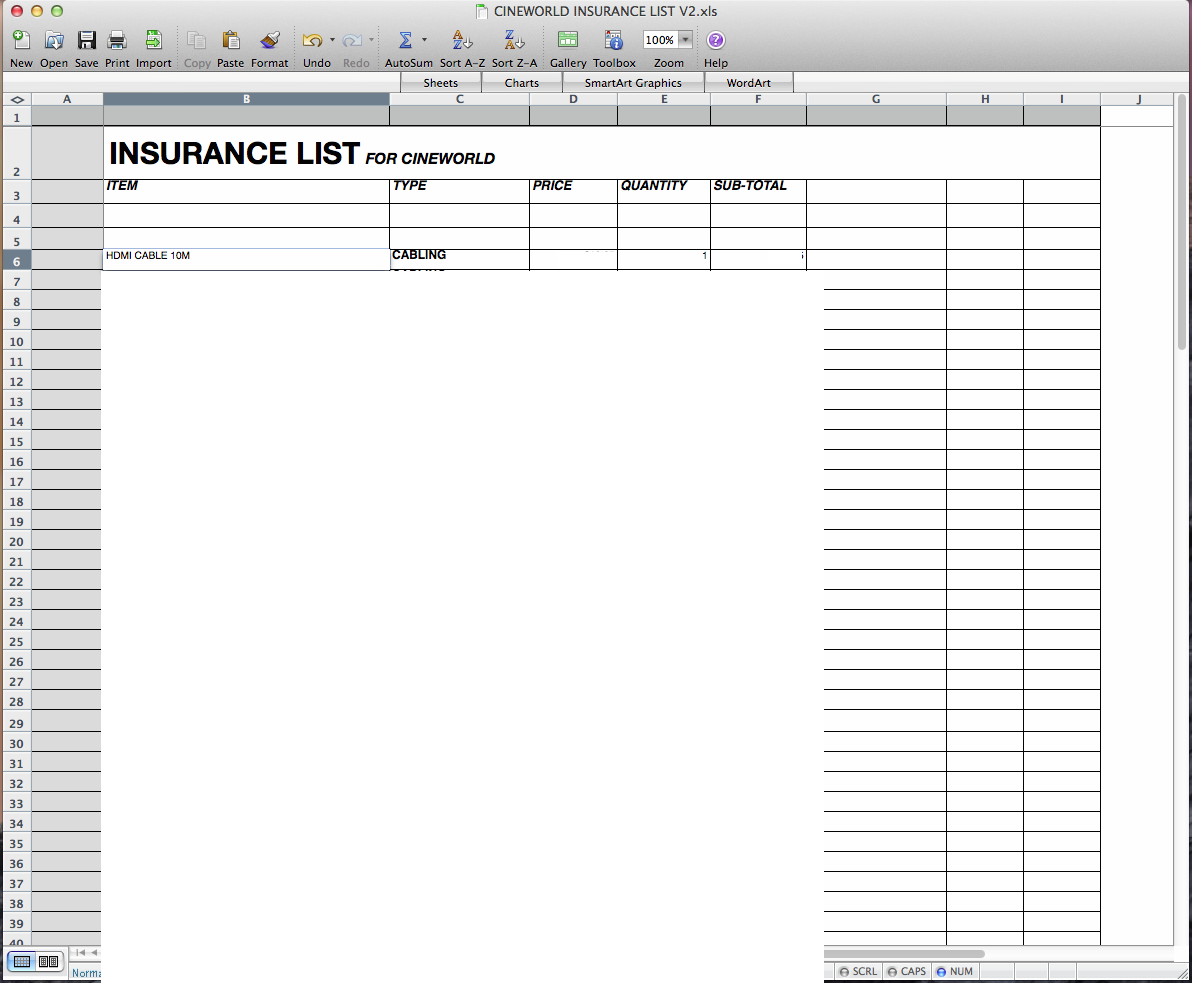
\includegraphics[width=\textwidth]{./Analysis/Forms/enter_data.png}
    \caption{Josh Entering Item Name.} \label{fig:print_function_result}
\end{figure}

\newpage

\noindent Here is an screen shot showing the calculation used to get the Sub-Total Value:

\begin{figure}[H]
    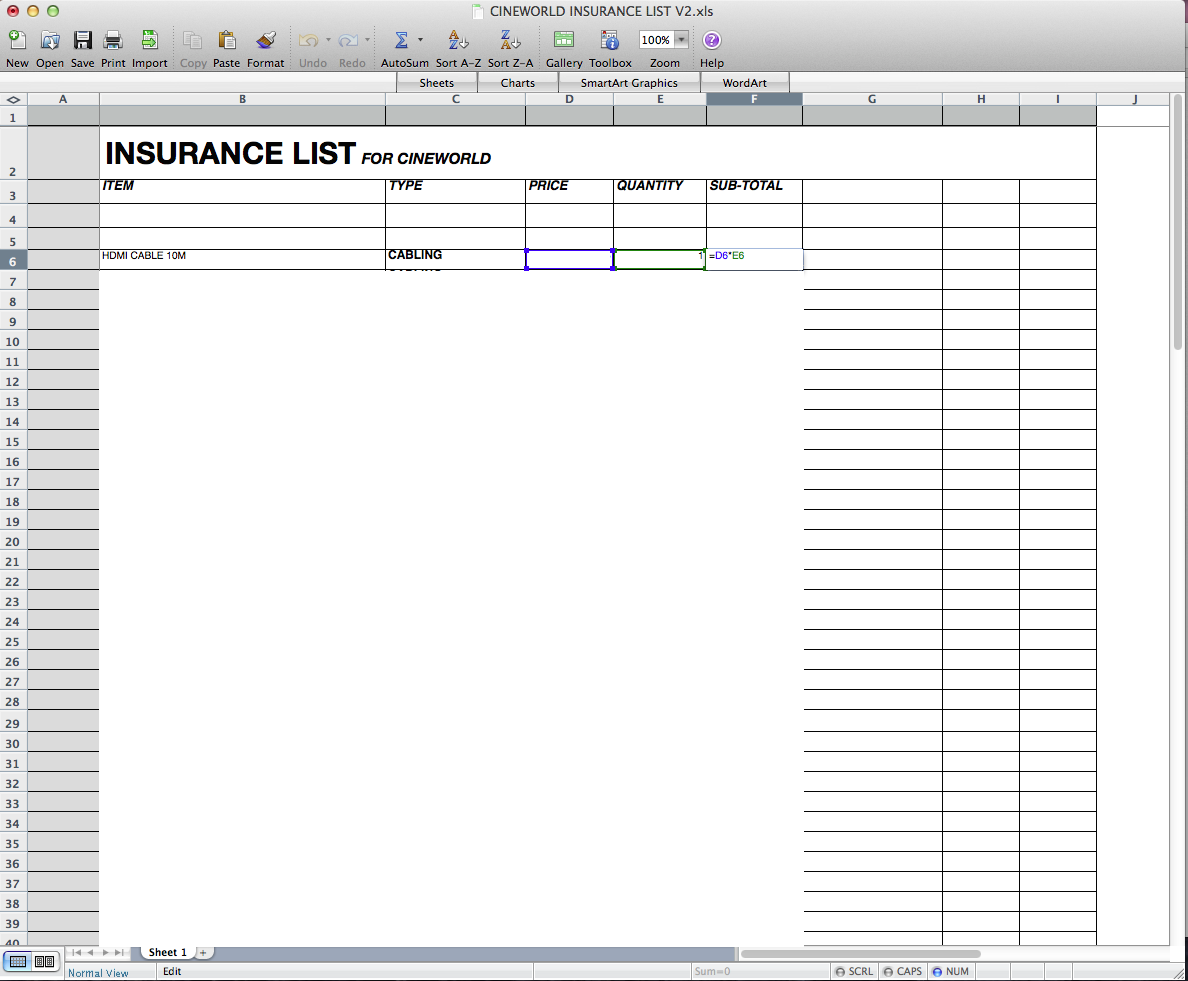
\includegraphics[width=\textwidth]{./Analysis/Forms/sub_total_calc.png}
    \caption{Sub-Total Calculation.} \label{fig:print_function_result}
\end{figure}

\subsection{The proposed system}

\subsubsection{Data sources and destinations}

The Following table shows the proposed data and their respective sources and destinations.

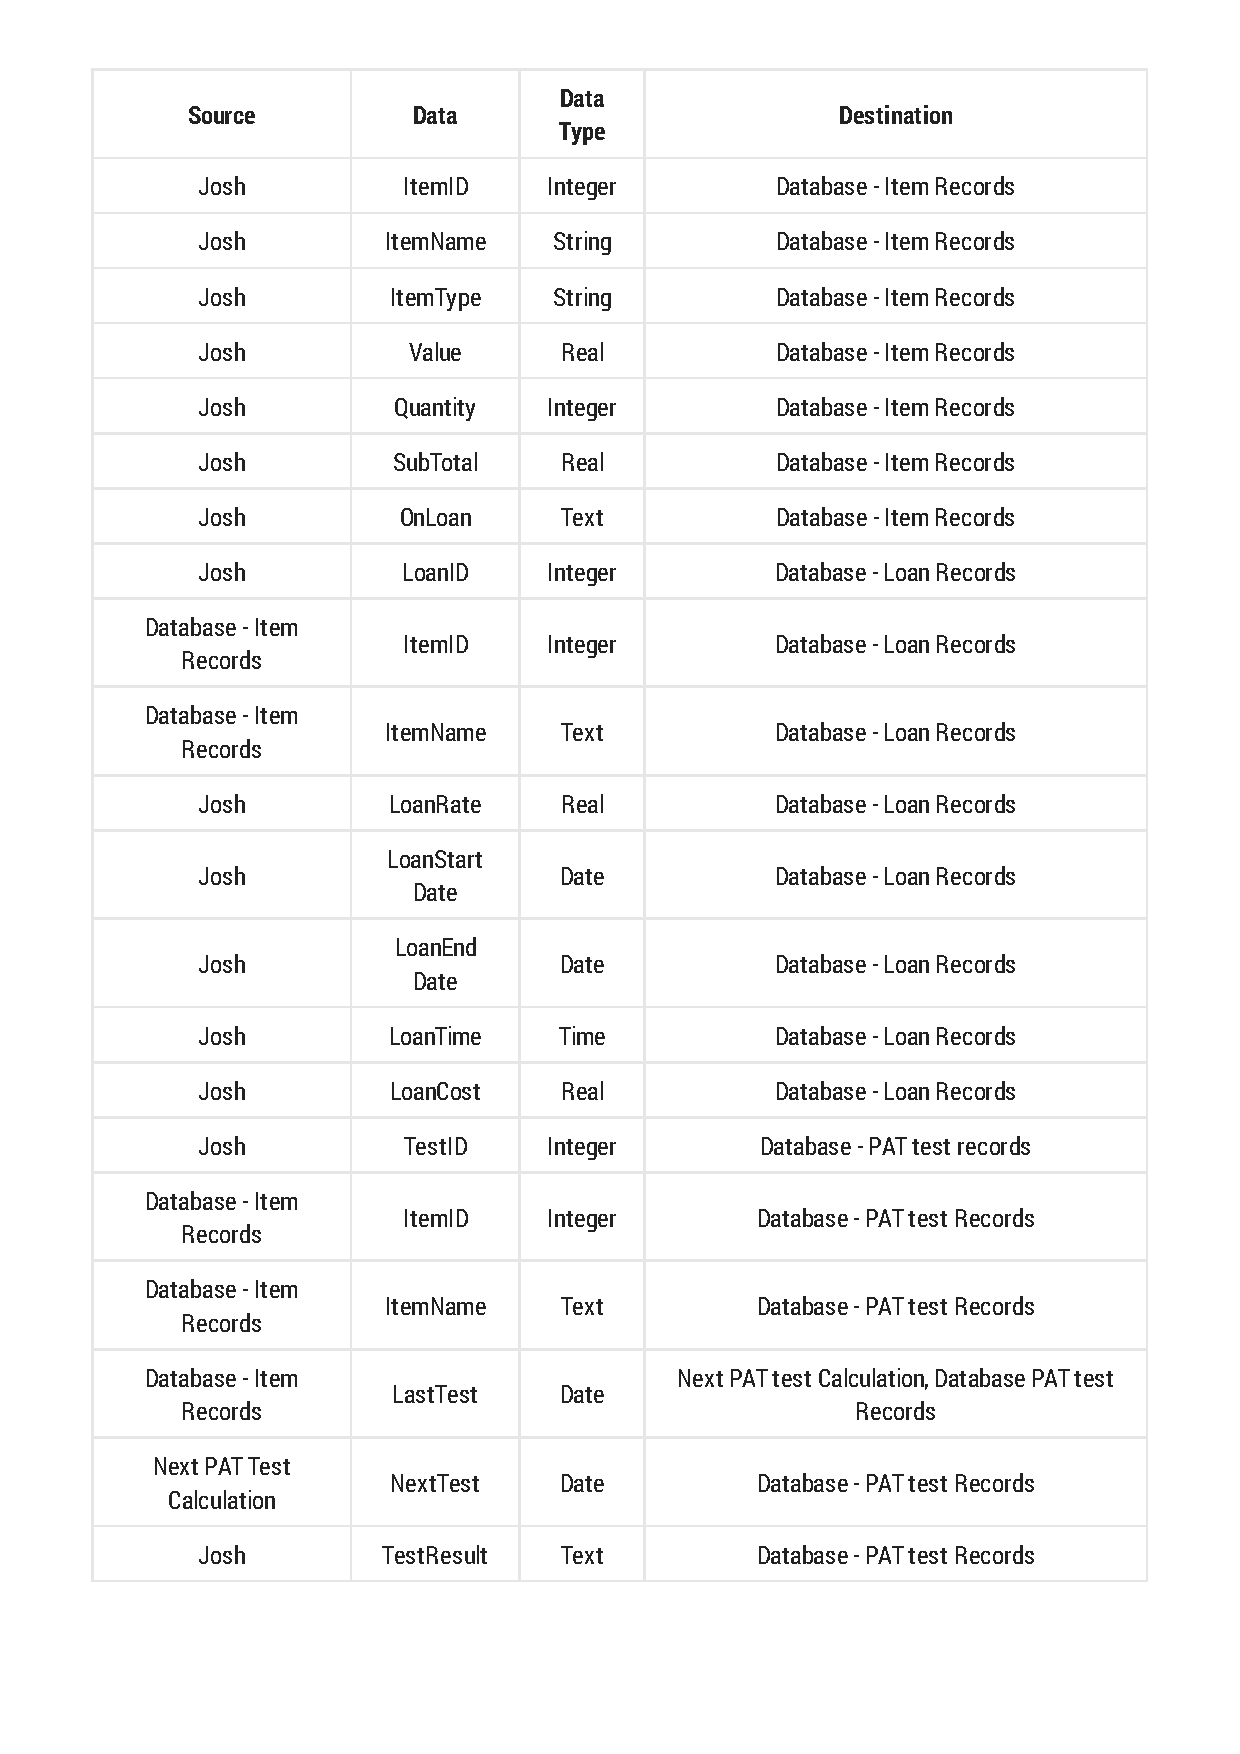
\includepdf[pages=-]{./Analysis/DataS&D/Data_S&D.pdf}


\subsubsection{Data flow diagram}

\begin{figure}[H]
    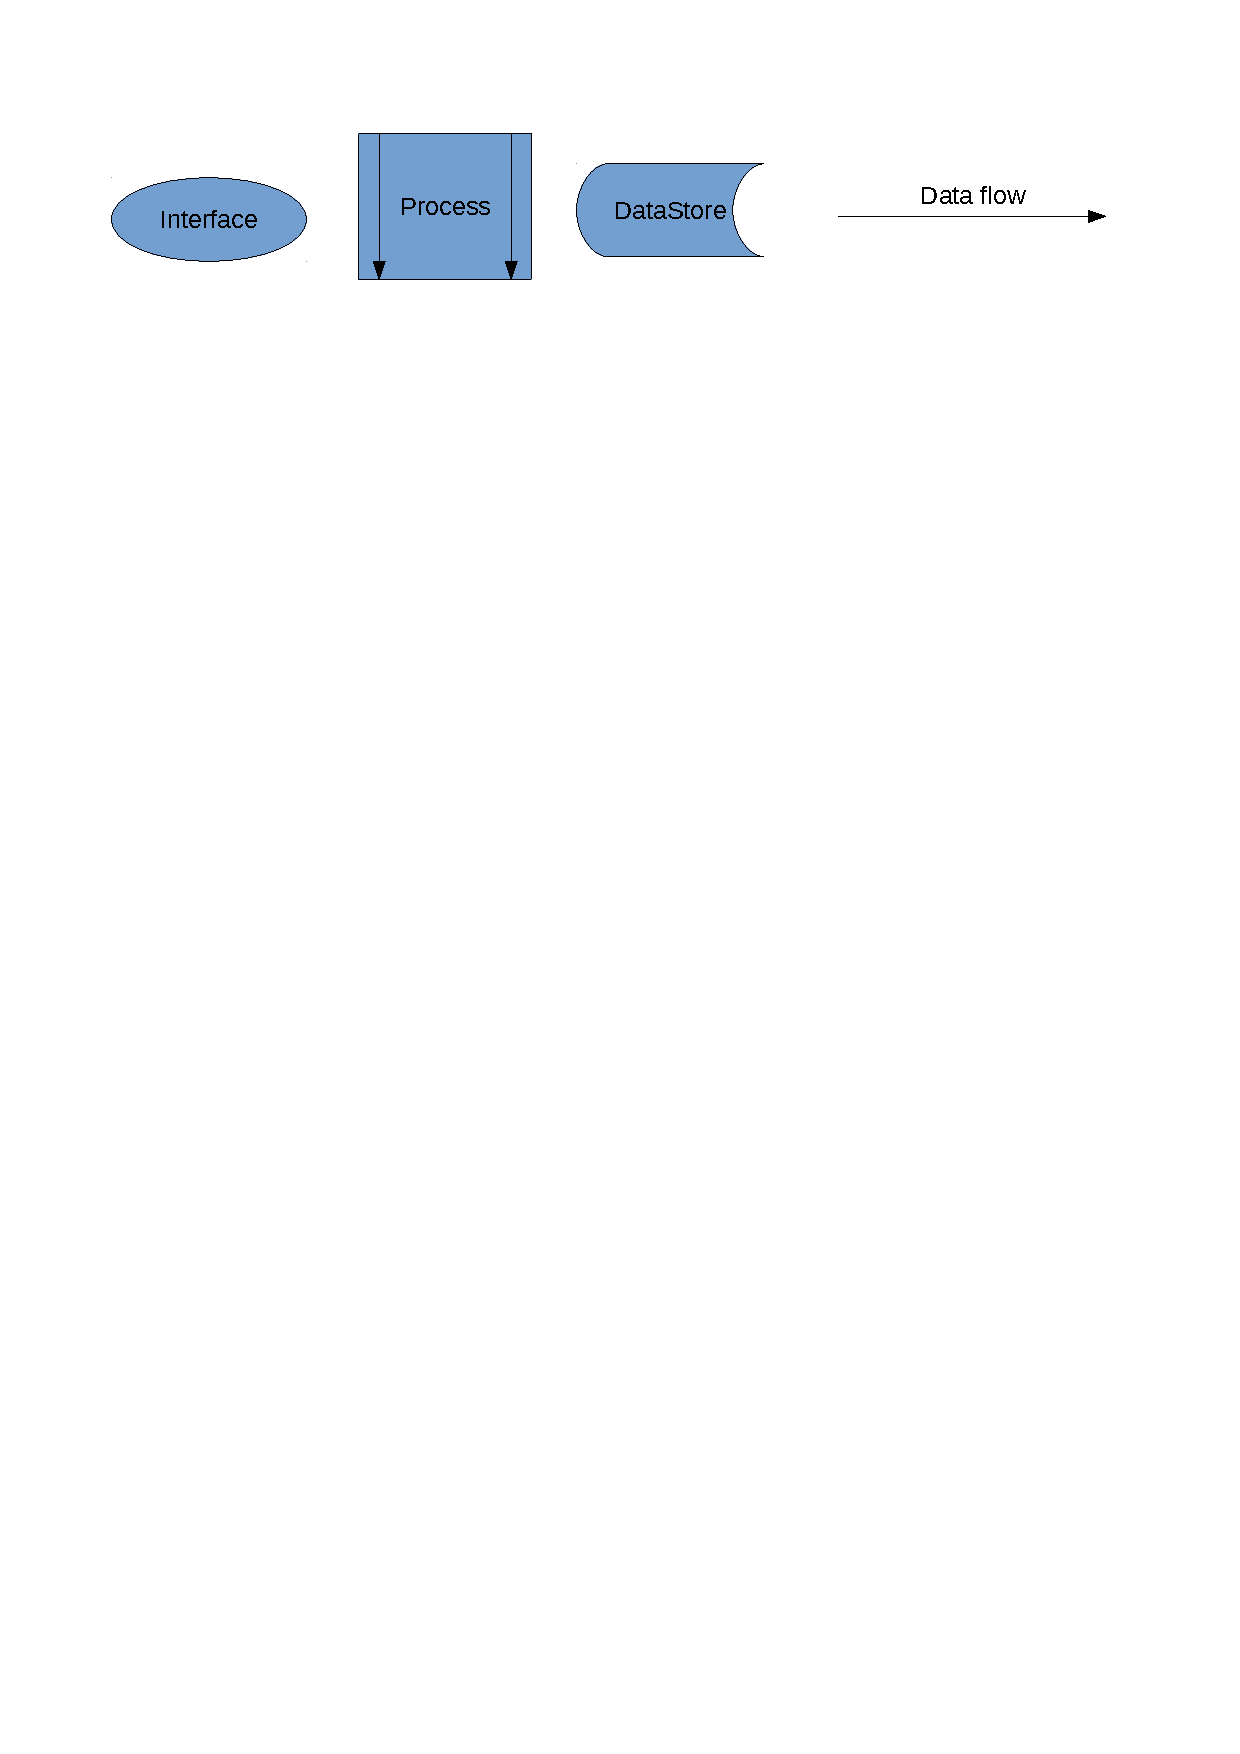
\includegraphics[width=\textwidth]{./Analysis/Dataflow/DFD_analysis_key.pdf}
    \caption{Flow Diagram Key.} \label{fig:print_function_result}
\end{figure}

\begin{figure}[H]
    \caption{Enter New Item.} \label{fig:print_function_result}
    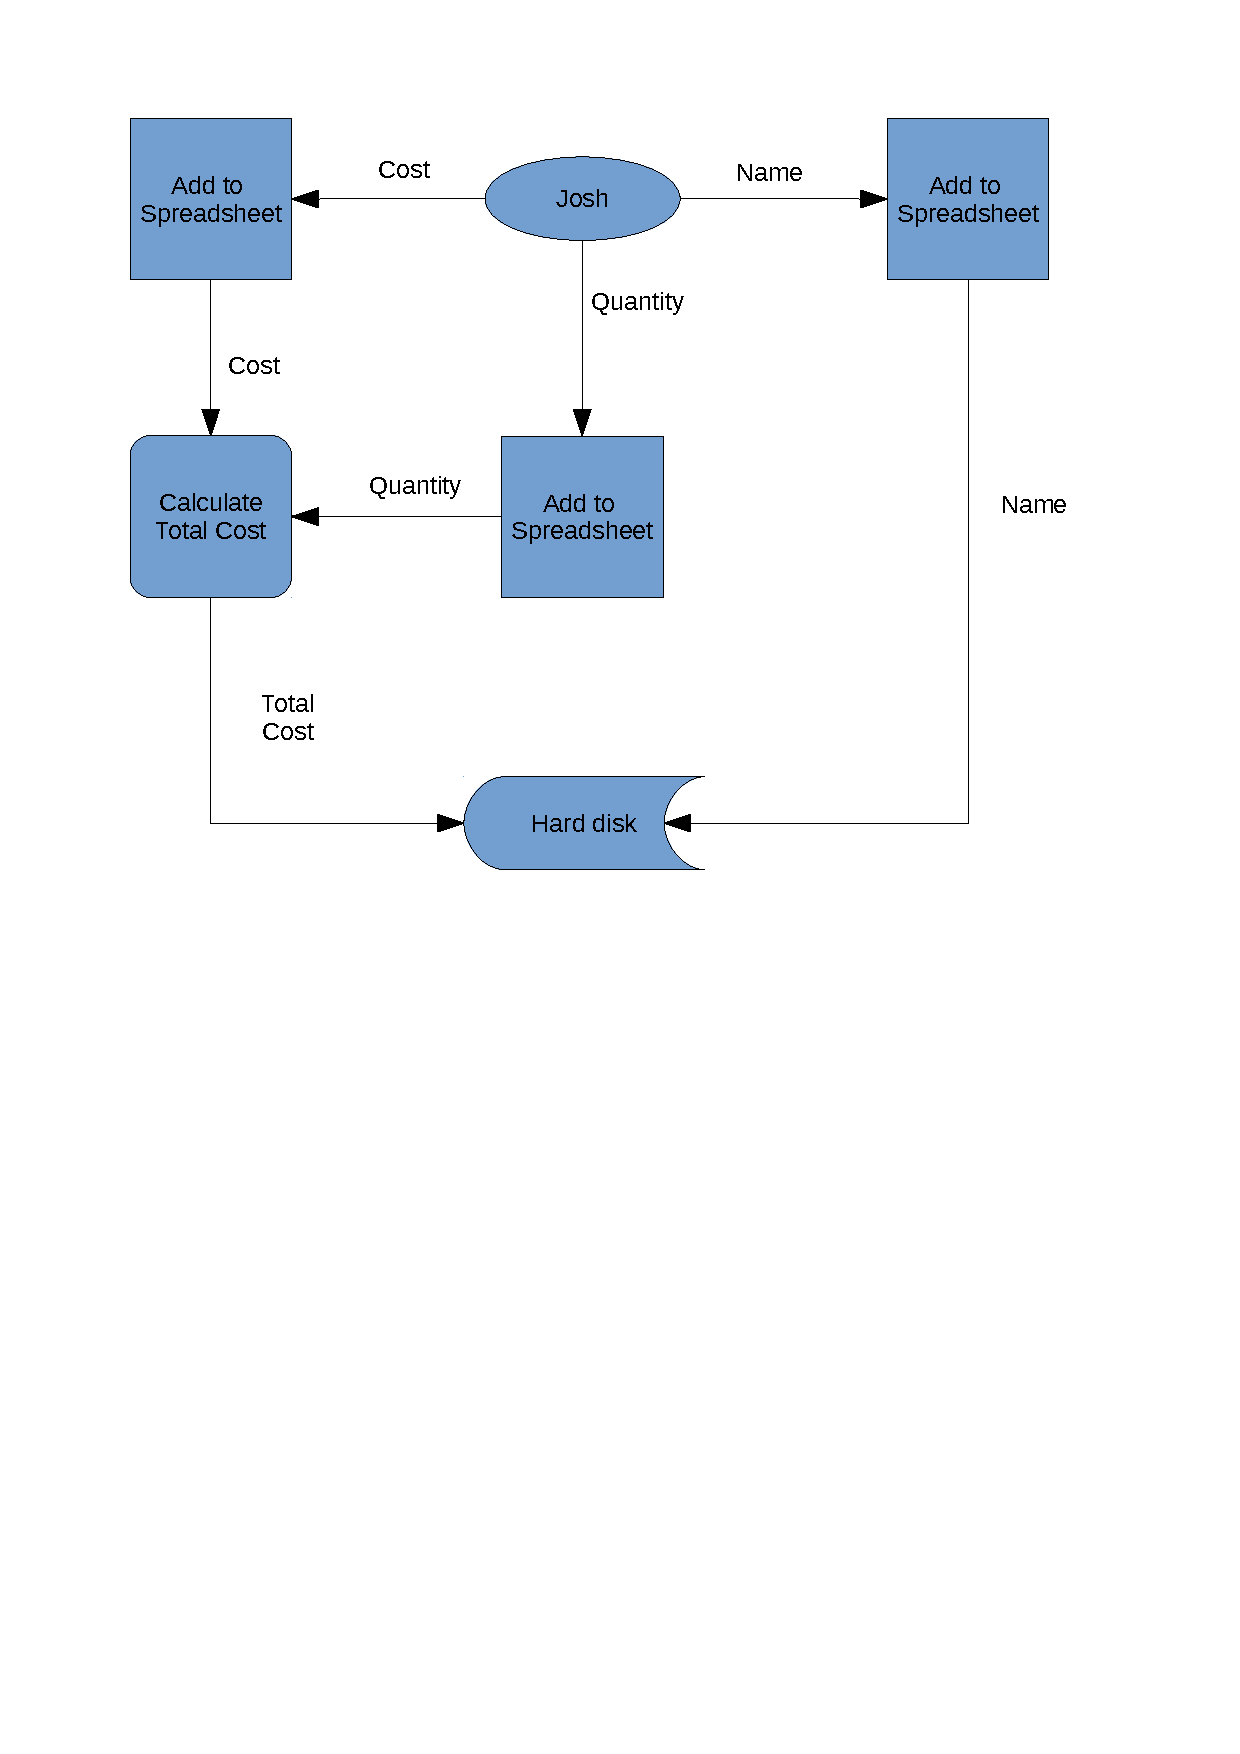
\includegraphics[width=\textwidth]{./Analysis/Dataflow/Data_flow_new.pdf}
\end{figure}

\begin{figure}[H]
    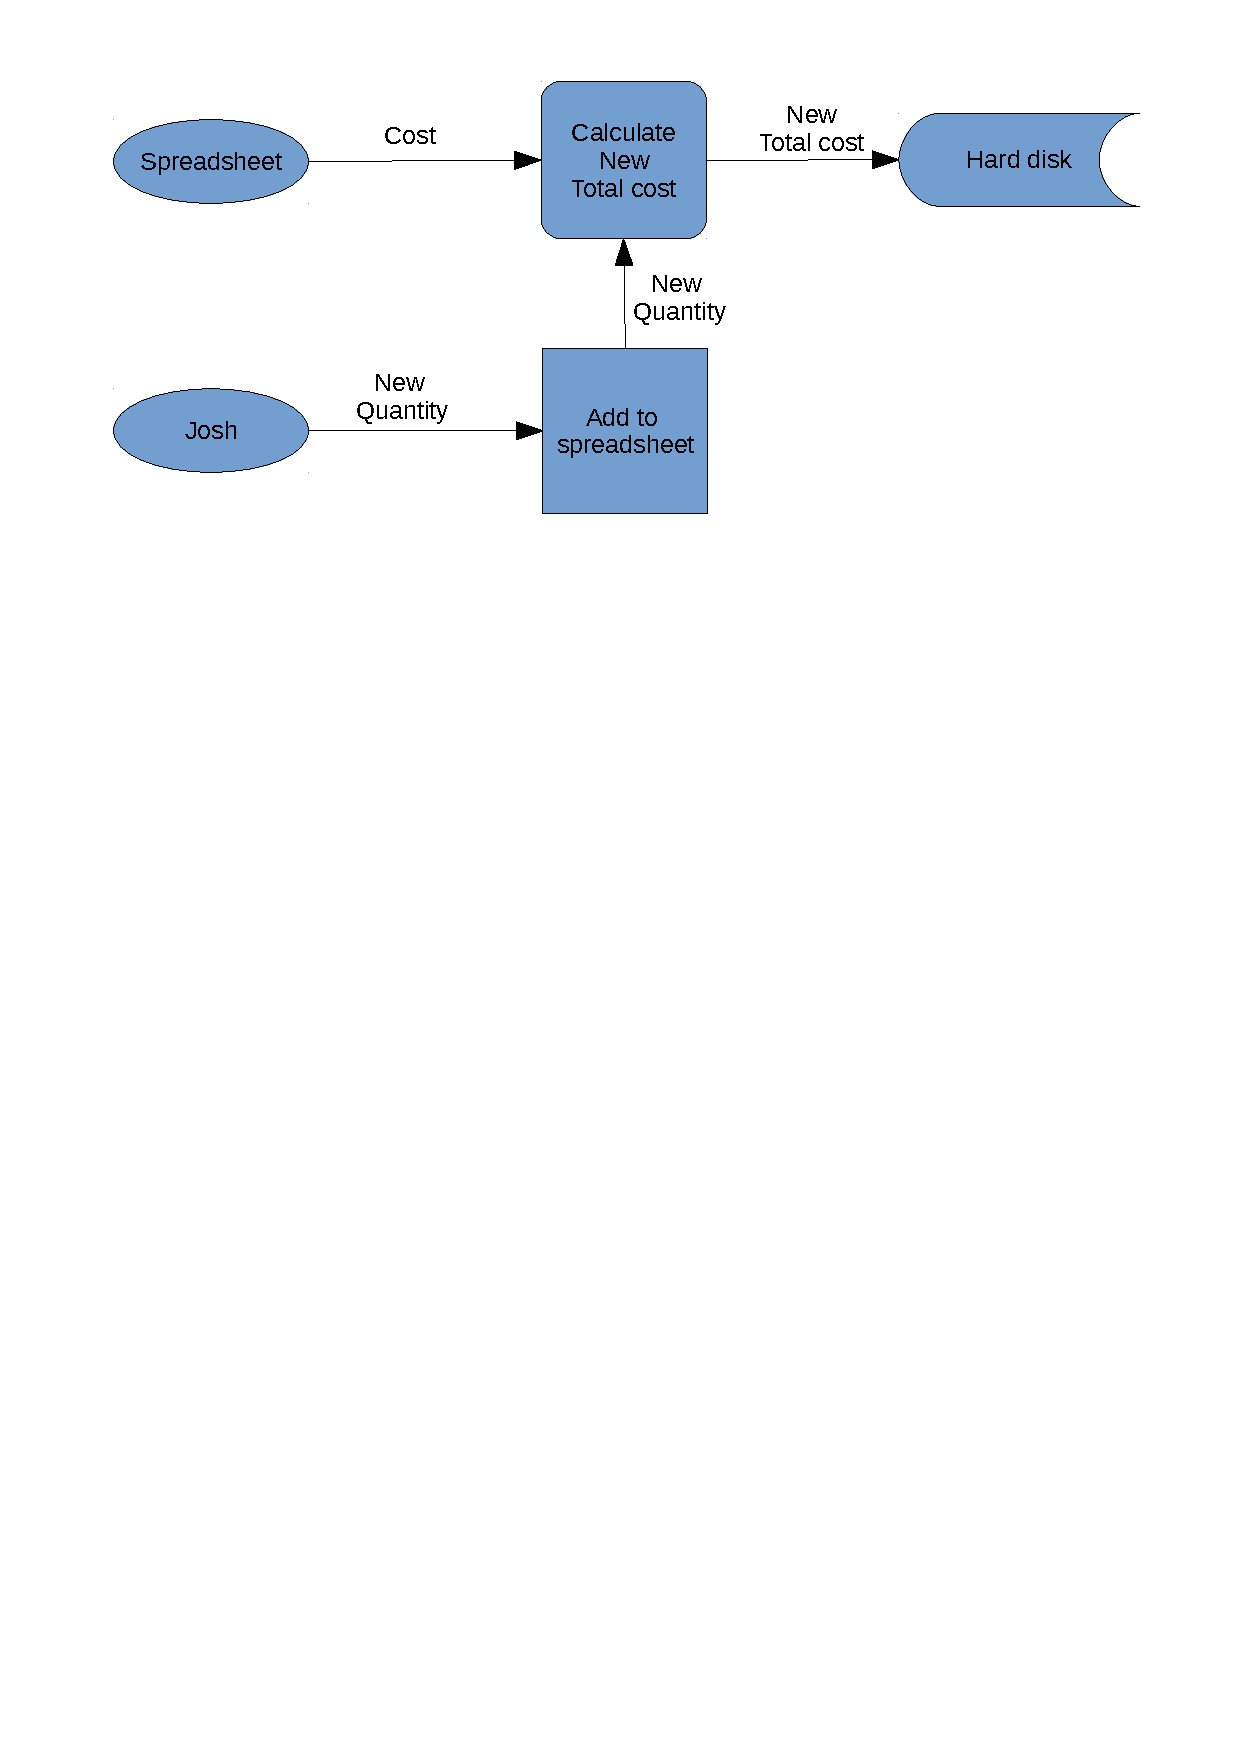
\includegraphics[width=\textwidth]{./Analysis/Dataflow/Data_flow_update.pdf}
    \caption{Enter New Item.} \label{fig:print_function_result}
\end{figure}



\subsubsection{Data dictionary}

\begin{figure}[H]
    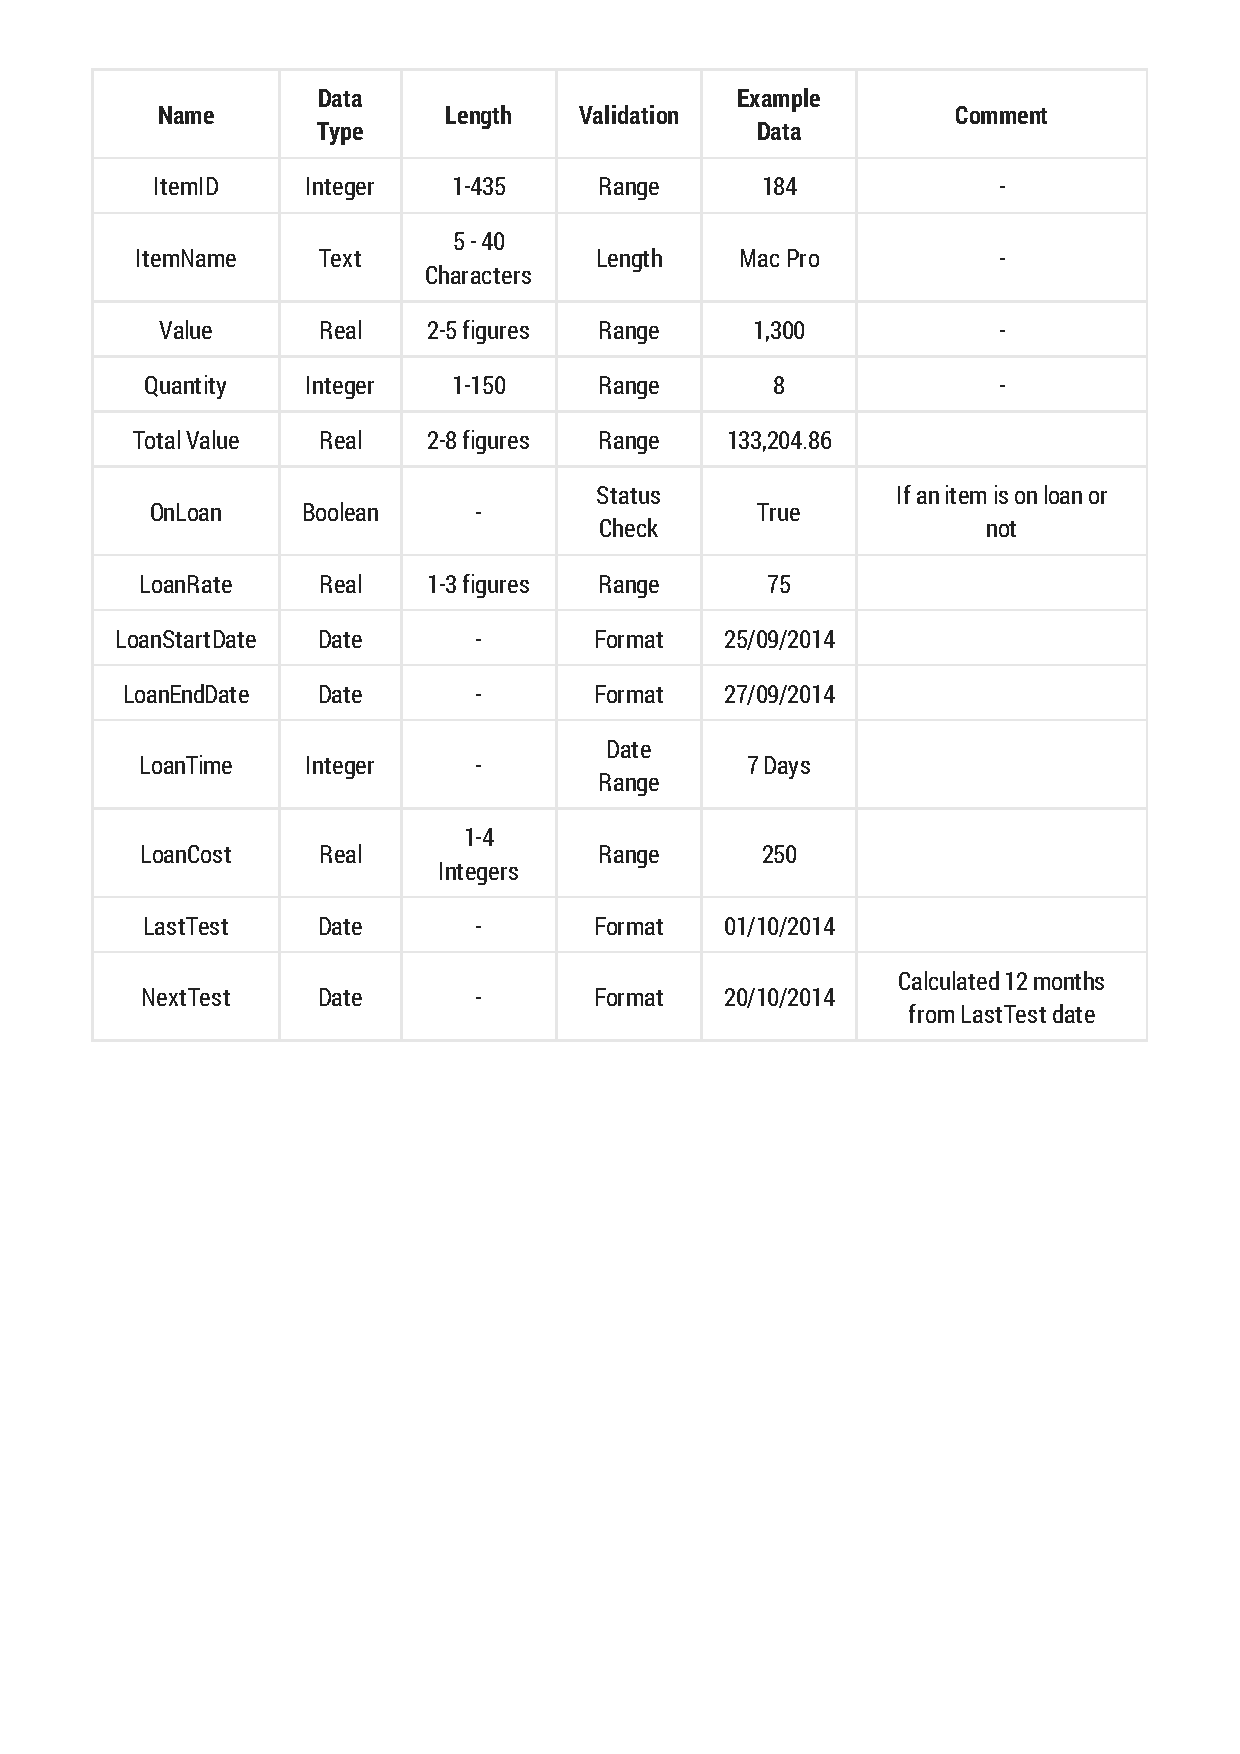
\includegraphics[width=\textwidth]{./Analysis/Dictionary/Data_dictionary.pdf}
    \caption{Data Dictionary.} \label{fig:data_dictionary}
\end{figure}

\newpage

\subsubsection{Volumetrics}

I have chosen to start off with only 20 Item Records along with 20 Loan Records and 20 PAT Test Records. In total there will be 60 Records.  I have chosen this number of records as my Client and I had previously agreed that this would be a suitable number of records to start with in order for him to get used to the system and train up other colleagues to know how to use it also. This can be increased as time goes by.\\

\noindent The Item Records Database, Loan Records Database and the PAT Test Records Database will store 18 fields of combined data. Each field should take up 1KB of hard disk space. With this the required initial storage space will be:

18KB * 60 = 1080KB

1080KB / 1024 = 1.05MB

If the rest of database managemnent system took up 28MB, the client would need 19.05MB of space for 60 records, with 18 fields of data

\section{Objectives}

\subsection{General Objectives}

\begin{itemize}
	\item Easily understandable layout and structure for records.
	\item Easy structure for input and outputs.
	\item Easy viewing of records
\end{itemize}

\subsection{Specific Objectives}

Record viewing:
\begin{itemize}
    \item Clear labels for data attributes.
    \item Next and Preious record buttons.
    \item Edit button so data cannot be changed accidentally.
    \item Submit button to save data changes (if any) to the current record.
    \item First and Last record buttons to jump to respective record.
\end{itemize}

\noindent Data input:
\begin{itemize}
    \item Data fields become editable
    \item Drop down selection for location selection
    \item Changes saved immediately after editng has finished (ie submit button pressed)
\end{itemize}

\noindent Data output:
\begin{itemize}
    \item Print button and functionality
    \item Export records to PDF
    \item Print/Export a batch of records to PDF
    \item Email notifications when new item is entered into database or an item is updated, the details and who entered/updated.
\end{itemize}


\subsection{Core Objectives}

\begin{itemize}
    \item Viewing of Item/Loan/PAT-test Records
    \item Item/Loan/PAT-test data input
    \item Item/Loan/PAT-test data editing
    \item Sending of Loan Invoices
\end{itemize}

\subsection{Other Objectives}

\begin{itemize}
    \item Printing records/invoices
    \item Exporting records/invoices to PDF
\end{itemize}

\section{ER Diagrams and Descriptions}

\subsection{ER Diagram}

\begin{figure}[H]
    \centerline{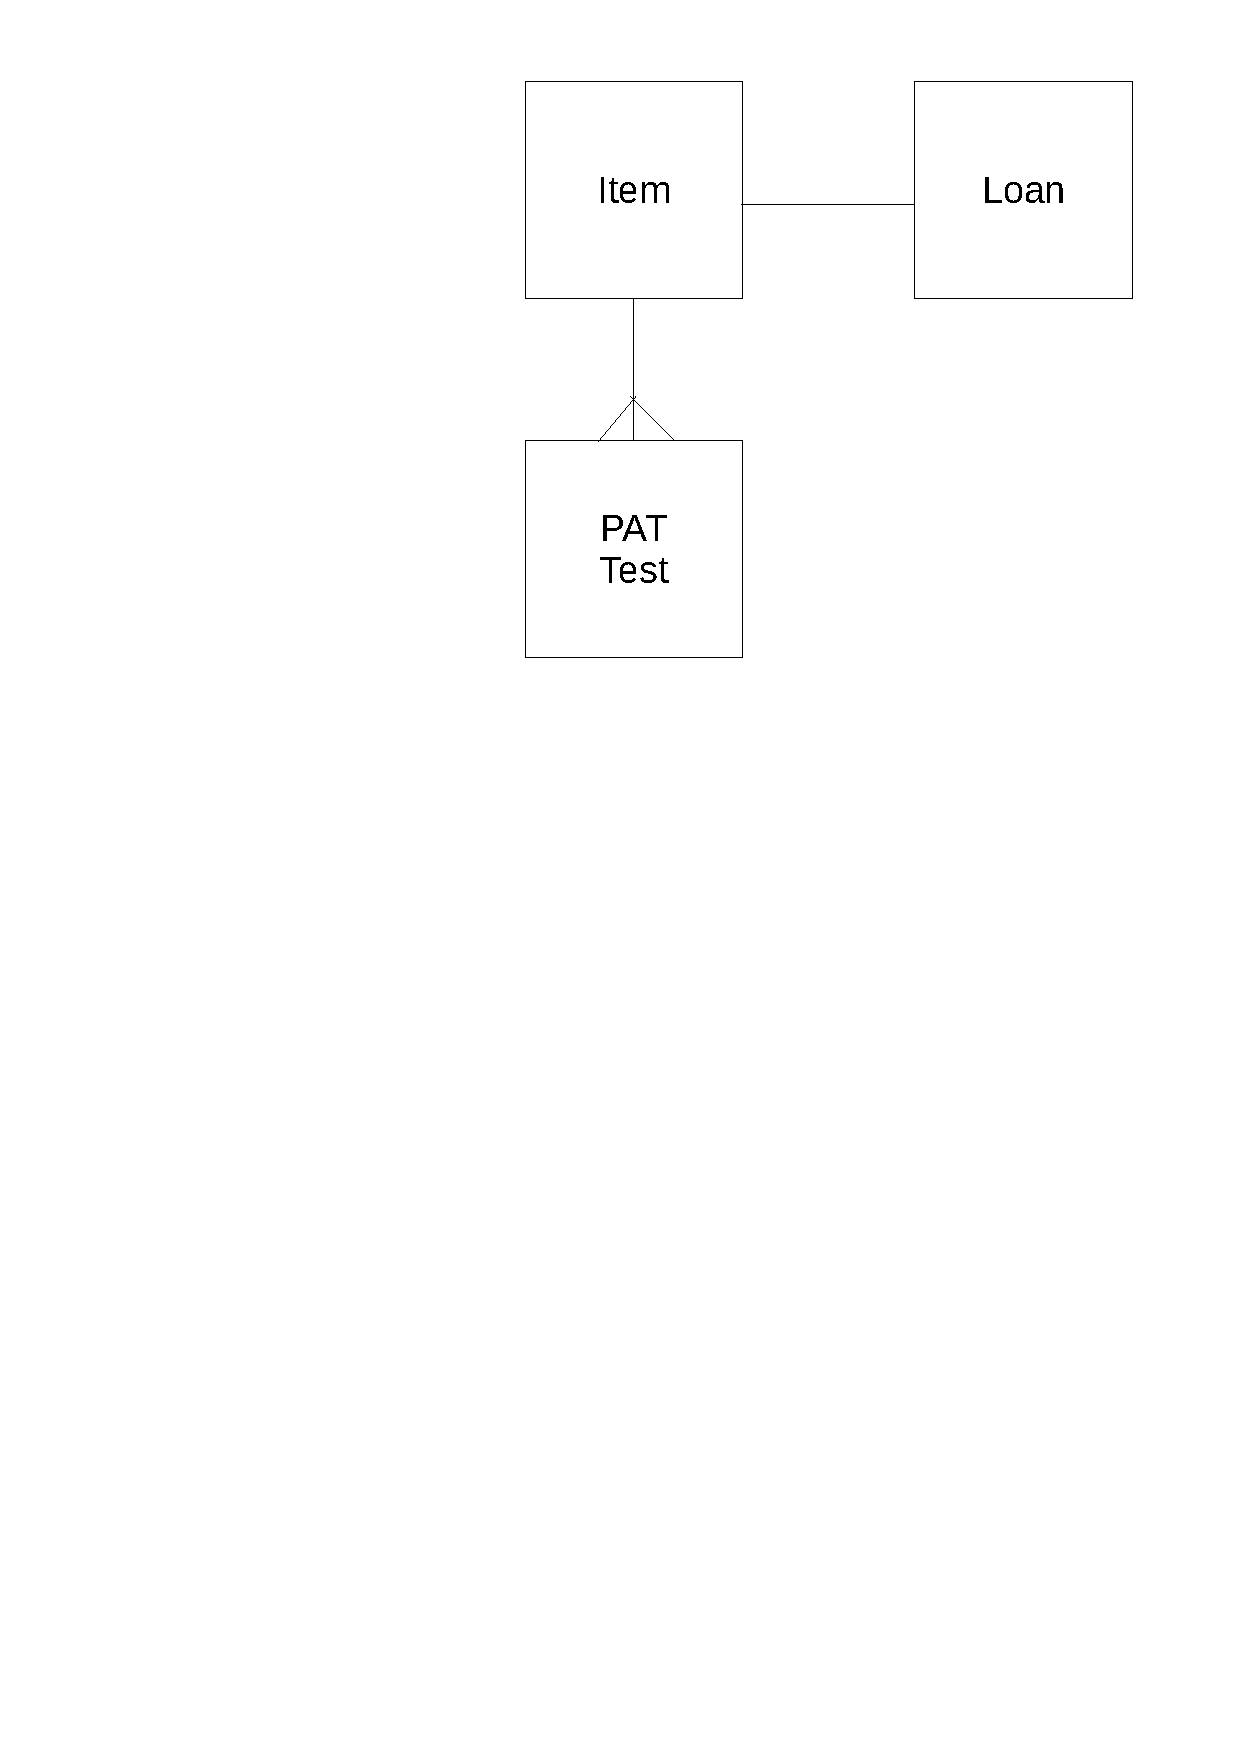
\includegraphics[width=250px]{./Analysis/ER_Diagrams/ER_Diagrams.pdf}}
    \caption{ER Diagrams.} \label{fig:ER Diagrams}
\end{figure}

\newpage

\subsection{Entity Descriptions}

Item(\underline{ItemID}, Name, Location, Value, Quantity, SubTotal, OnLoan,\\
\noindent \emph{PATNeeded})\\

\noindent Loan(\underline{LoanID}, \emph{ItemID}, \emph{ItemName}, LoanRate, LoanStartDate, LoanEndDate, LoanTime, LoanCost)\\

\noindent PATTest(\underline{TestID}, \emph{ItemID}, \emph{ItemName}, LastTest, NextTest)

\section{Object Analysis}

\subsection{Object Listing}

\begin{itemize}
    \item Client
    \item Item
    \item Loan
    \item PAT test
\end{itemize}

\subsection{Relationship diagrams}

\begin{figure}[H]
    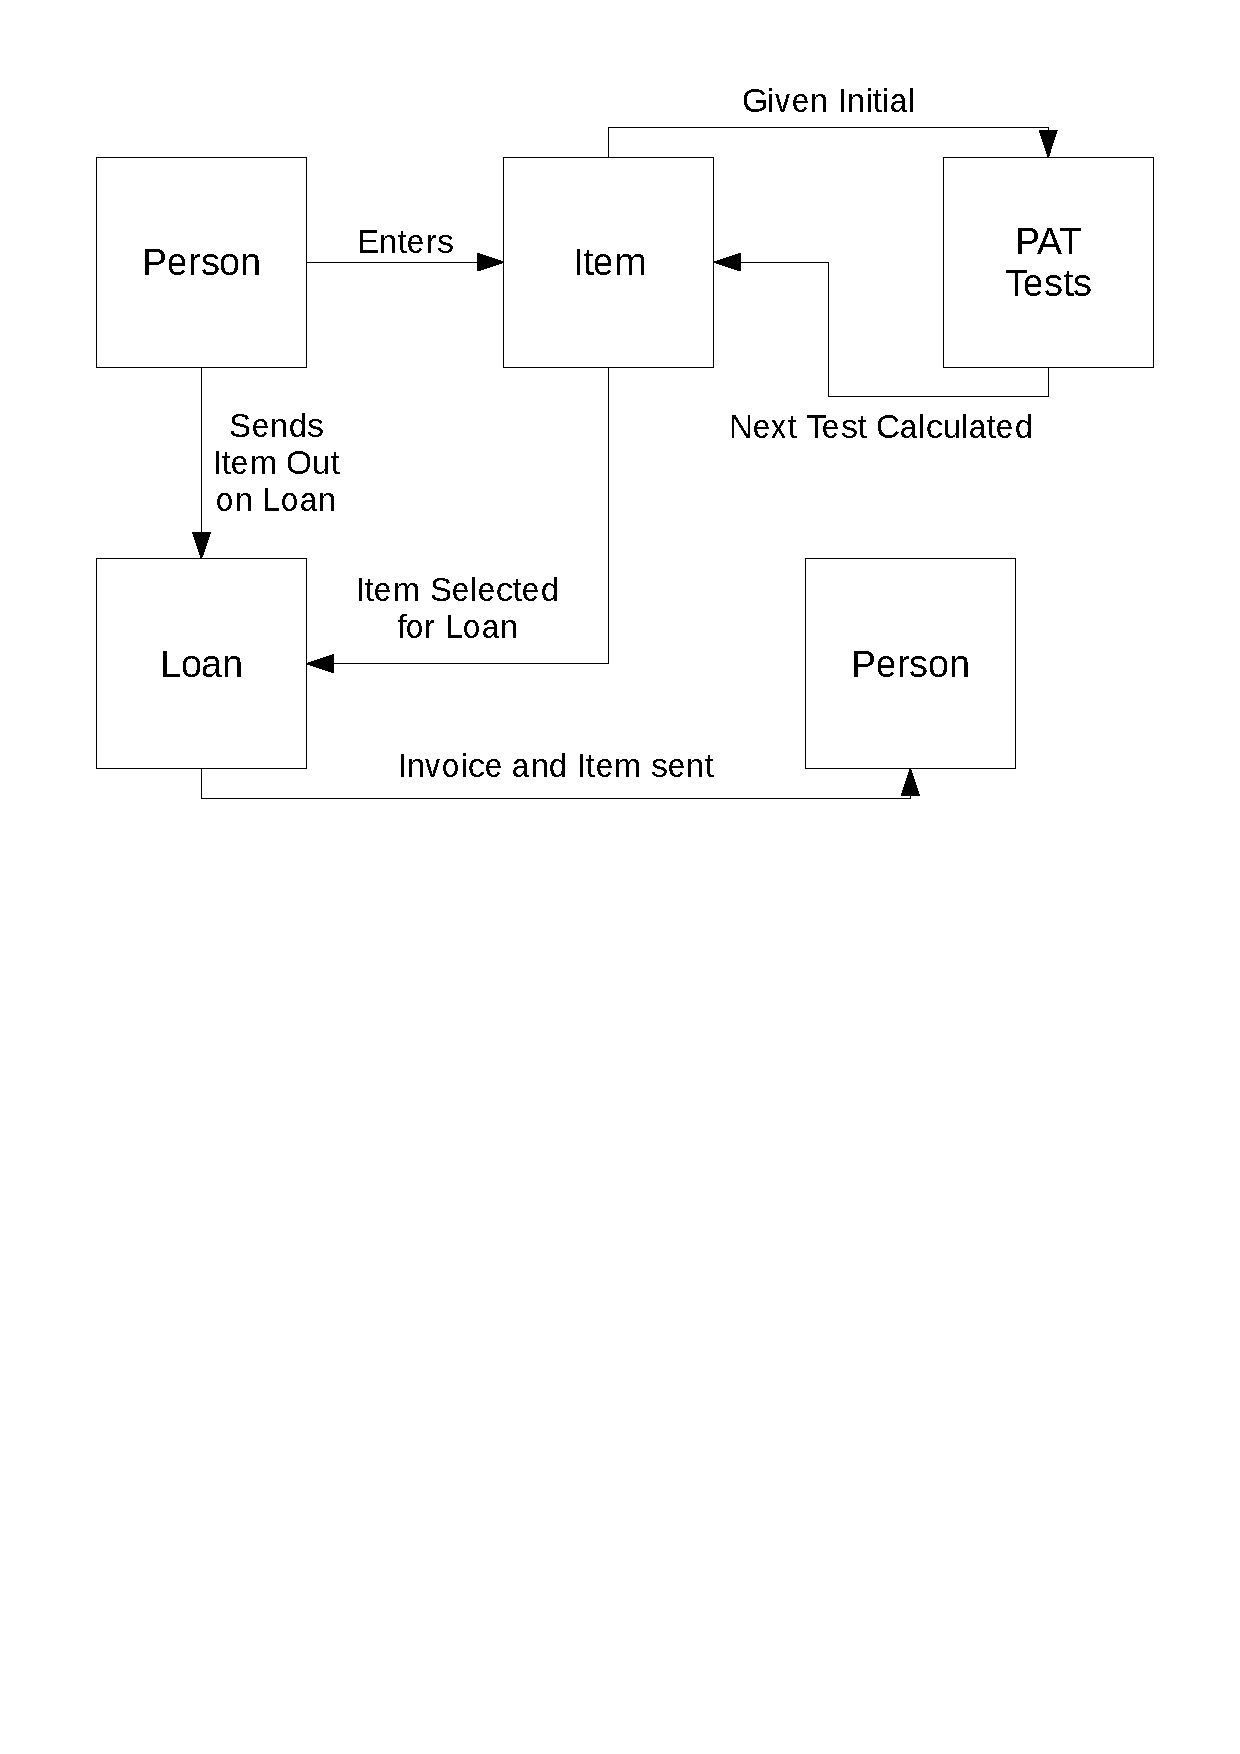
\includegraphics[width=\textwidth]{./Analysis/Relationship_Diagrams/Relationships_diagrams.pdf}
    \caption{Relatioship Diagram.} \label{fig:relationship_diadram}
\end{figure}

\newpage

\subsection{Class definitions}

\begin{figure}[H]
    \centerline{\includegraphics[width=100px]{./Analysis/Class_Definitions/Class_definition_key.pdf}}
    \caption{Class Diagram Key.} \label{fig:relationship_diagram}
\end{figure}

\begin{figure}[H]
    \centerline{\includegraphics[width=\textwidth]{./Analysis/Class_Definitions/Class_diagrams.pdf}}
    \caption{Class Diagrams.} \label{fig:relationship_diagram}
\end{figure}

\newpage

\section{Other Abstractions and Graphs}

\section{Constraints}

\subsection{Hardware}

Presently, Josh uses a custom built, 2008 MacPro Desktop Computer. This is primarily used as a file server for images, audio and video files a well as a backup for his current work desktop. My system will need to be compatible with this system.\\

\noindent Computer Specifications:
\begin{itemize}
    \item 2x 2.8 GHz Quad-Core Intel\textregistered Xeon\texttrademark Processor
    \item ATI Radeon HD 2600 XT 256MB Graphics Card
    \item 661-4449 Apple Mac Pro A1186 Motherboard
    \item 16.00GB DDR3 RAM
    \item 1TB SATA Disk-Drive
    \item 6TB RAID Storage
    \item Apple SuperDrive
    \item 15" LG E1942 LCD Display. 1280 x 720 pixels
\end{itemize}

\noindent The proposed system should have little to no impact on this machine as the processing power and memory that can be disipated by the computer, greatly excedes the requirements for the proposed system.\\

\noindent There are, however, a few hard constraints that will have to be considered. One of which is the resolution of the display. The proposed system will have to be designed and implemented by taking this into account, otherwise the system may not fit the screen size appropriately.\\

\noindent One other constraint of the computer to be used is that it is a desktop computer. This means that the system is only accessible where Josh chooses to have the computer based in his place of work, as the computer is not portable. In addition to this, the computer requires a constant supply of power in order to opperate as there is not internal battery.\\

\subsection{Software}

Josh has told me that there little restriction as to what software can and can't be stalled. The only restriction in place is that I don't install pirated, illegal or damaging software on the machine as it is part of an inter network of systems and can be accessed by other computers. The current operating system in place is Apples OSX 10.8 (Mountain Lion). Josh wishes to update the software sometime in the near future to OSX 10.9 (Mavericks) and possibly update to OSX 10.10 (Yosemite) when a stable version has been released within the next 3-5 months.

\subsection{Time}

Josh has said that there is no deadline requirement for the proposed system to be in place and doesn't need it until I have finished implementing it. The only deadline I need to meet is the project deadline set by my Computing course leader. This is Friday 13 \textsuperscript{th} February 2014.

\subsection{User Knowledge}

Josh posses a qualification in A level Media studies as well as 2 years use of comuters during his degree. He has substantial understanding of how to use computers as his job requires he uses one most of the time. Josh also has required knowledge of how to use many variaties of applications. He uses Adobe Creative Suite for most of his job as he designs various forms of media. He also has knowledge of Apple's Final Cut Pro application as well as many others.\\

\noindent When designing and implementing the proposed system, Josh's experience with computers will have to be considered. Josh tends to use the internet browser Google Chrome for all his web-browsing and research as well as a third party mail application called. By designing the system similarly to these applications, it should make it easier to understand how the system works and get used to using it a lot faster than it would if the system had a primitive design.\\

\noindent There will also be a full manual included to aid Josh with learning and understaning the familiar interface, the functionality of the new system and how to use certain features.

\subsection{Access restrictions}

The proposed system is primarily to be accessed by Josh himself. However, he can see it being an advantage if other people had access to the system.\\

\noindent For this reason, we have agreed that having the database password protected is the best way fo Josh to control who can do what with the data. He will be able to distribute usernames and passwords to other colleagues who he feels should have different access levels (Admin or standard). This reduces the risk of records being deleted that shouldn't have been. It also allows Josh to monitor who has entered new data, or updated existing data.

\noindent Users should be able to change their passwords to a more memorable one when they log into the system for the first time.

\section{Limitations}

\subsection{Areas which will not be included in computerisation}

Initial buying of new items will not be included in the computerisation as this is still done either in person or over the world wide web. Similarly, intial sales of items will not be included in the computerisation, it will only be once the item has been bought/sold that the data will be updated to coincide with the quantity changes.

\subsection{Areas considered for future computerisation}

The process of an external client of Josh's buying and receiving an item could be included in the system as it would be easier to produce an invoice and quote sheet from the data already in the system rather than query the database and hand draft an email to be sent. The system could be included if I have time at the end and have the relevant knowledge in order to accomplish the task

\section{Solutions}

\subsection{Alternative solutions}



\textbf{Custom made database:}

Advantages
\begin{itemize}
    \item No need to install addidtional software, only a simple database management system such as "Microsoft Access" or "Filemaker".
\end{itemize}

Disadvantages
\begin{itemize}
    \item Database managment systems often cost a substantial amount of money for a license.\\
\end{itemize} \hline



\textbf{Web based application:}\\

Advantages
\begin{itemize}
    \item Easily accessible by other users. Doesn't rely on one machine.
    \item Can have 'Cloud based' storage of files.
    \item More than one user can be logged on at a time.
\end{itemize}

Disadvantages
\begin{itemize}
    \item Website or server hosting can be expensive.
    \item More advanced security methods will be required due to the system being constantly online and therefore vulnerable to attack.
    \item Better networking knowledge required to compensate for the security implications and risks.\\
\end{itemize}\hline

\newpage

\textbf{Terminal or Command based application:}\\

Advantages
\begin{itemize}
    \item More power efficient as it isn't graphics heavy, much easier to desgin as the interface is just text.
    \item Fast efficient opperation provided the client has knowledge of terminal and shell commands.
\end{itemize}

Disadvantages
\begin{itemize}
    \item Careful error handeling needed as the user could enter any known/valid command.
    \item Training is required so that the client knows what commands to use when.
    \item There are often commands that the client don't know about that could potentially corrupt his computer.\\
\end{itemize}\hline



\textbf{Python destop application with a GUI:}\\

Advantages
\begin{itemize}
    \item Designed and layout can be client specific.
    \item Minimal error with radio buttons and other widgets.
    \item Easy to understand layout as data can be formatted to fit the clients requirements.
    \item Easy to visualise what is happening with graphs and tables.
\end{itemize}

Disadvantages
\begin{itemize}
    \item More time needed to build the interface and sql database compaired to a command based application.
    \item More resources needed from the computer for graphical visualistaion and database storage 
    \item Programming the graphical interface could prove a difficult task\\
\end{itemize}\hline


\subsection{Justification of chosen solution}


I have chosen to use the \emph{'Python Desktop Application with a GUI'} solution. \\

\noindent These are my reasons:

\begin{itemize}
    \item The application takes up no physical space apart from the computer it is installed on.
    \item I already have the required language knowledge needed to program a database and a GUI in Python
    \item Using a custom made desktop application is faster for Josh to manage his inventory than the current spreadsheet based system.
    \item Backup can be made and data can be restored easily in the event of corruption or unresolvable data loss
\end{itemize}
